% !TEX root = ..\thesis.tex


\chapter{ĐOẠN CỦA QUANH}

////////////Thiếu cái hình DECODER nha

\section{Setup Gateway}
\subsection{Access LG02}
Cấp nguồn điện cho gateway, sau đó dùng laptop để bật scan wifi, lúc này sẽ xuất hiện tên wifi : “dragino-168cb0”

Kết nối với wifi đó và truy cập địa chỉ IP: “10.130.1.1”, lúc này sẽ đến giao diện để configure gateway bằng cách nhập username và password như hình \ref{fig:gateway_configure}
\begin{figure}[H]
    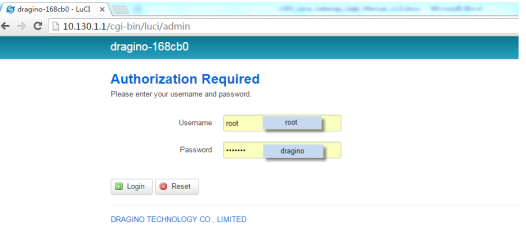
\includegraphics[width=\textwidth]{images/Quanh/Gateway_configure.png}
    \caption{Xác thực tại địa chỉ 10.130.1.1}
    \label{fig:gateway_configure}
\end{figure}

\subsection{Cài đặt network}
Truy cập Internet như Wifi Client theo các bước:
\begin{description}
    \item Bước 1: Network → Wireless, chọn radio0 và scan như hình \ref{fig:radio0_scan}
    \begin{figure}[H]
        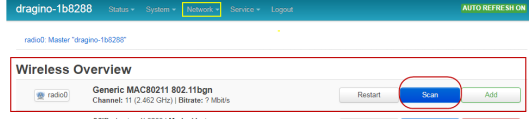
\includegraphics[width=\textwidth]{images/Quanh/Radio_scan.png}
        \caption{Scan mạng Wireless}
        \label{fig:radio0_scan}
    \end{figure}
    
    \item Bước 2: Chọn wifi và tham gia vào mạng, sau đó nhập mật khẩu và Submit như hình \ref{fig:join_password}
    \begin{figure}[H]
        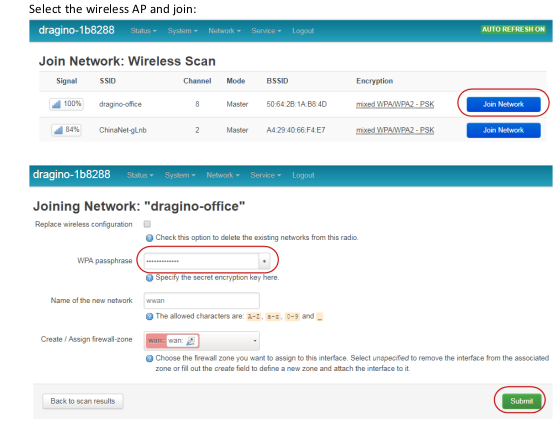
\includegraphics[width=\textwidth]{images/Quanh/Join_password.png}
        \caption{Tham gia vào wifi và nhập mật khẩu}
        \label{fig:join_password}
    \end{figure}
    \item Bước 3: Network → Wireless, chọn disable wifi mặc định của gateway như hình \ref{fig:disable_wifi}
    \begin{figure}[H]
        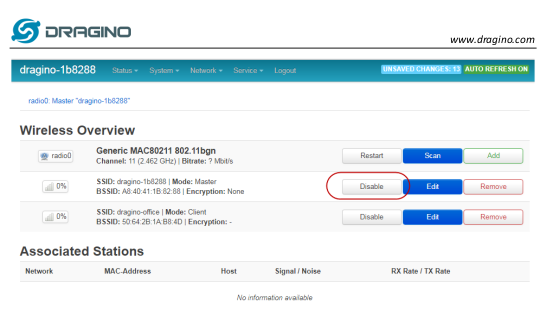
\includegraphics[width=\textwidth]{images/Quanh/Disable_wifi.png}
        \caption{Tắt wifi mặc định}
        \label{fig:disable_wifi}
    \end{figure}
\end{description}
(lưu ý, sau khi thực hiện bước 3, kết nối sẽ bị mất, nếu laptop kết nối wifi mặc định lúc nãy)

Trong trường hợp không thể truy cập địa chỉ 10.130.1.1 nữa, ta sử dụng cổng LAN để kết nối:
\begin{enumerate}
    \item Kết nối LAN Port
    \item Configure Ethernet port có địa chỉ IP như hình \ref{fig:config_ethernet}
    \begin{figure}[H]
        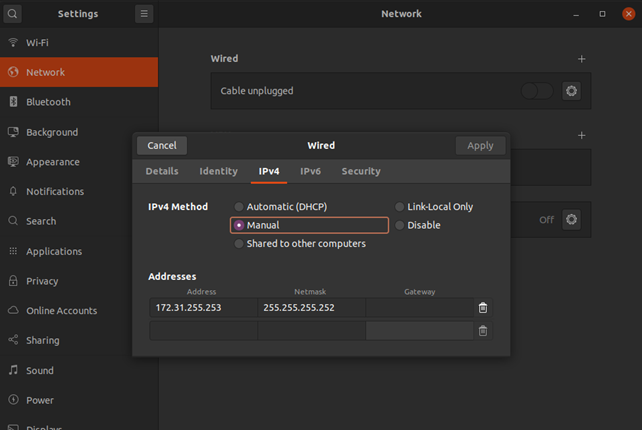
\includegraphics[width=\textwidth]{images/Quanh/Config_ethernet.png}
        \caption{Cấu hình địa chỉ IP của cổng Ethernet (Ubuntu 20.04)}
        \label{fig:config_ethernet}
    \end{figure}
    \item Dùng địa chỉ 172.31.255.254 để truy cập vào Web
\end{enumerate}

\subsection{Tạo gateway trên TTN Server}
\begin{description}
    \item Bước 1: Vào Service → LoRa → Lấy ID của Gateway như hình \ref{fig:get_gateway_id}
    \begin{figure}[H]
        \centering
        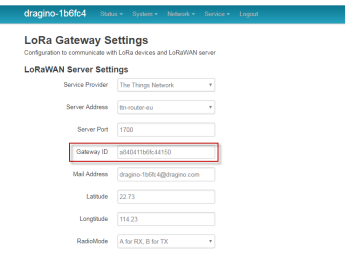
\includegraphics[width=\textwidth]{images/Quanh/Gateway_ID.png}
        \caption{Lấy ID của Gateway}
        \label{fig:get_gateway_id}
    \end{figure}
    \item Bước 2: Truy cập TTN: https://console.thethingsnetwork.org/gateways, giao diện hiển thị ở hình \ref{fig:gateway_console}
    \begin{figure}[H]
        \centering
        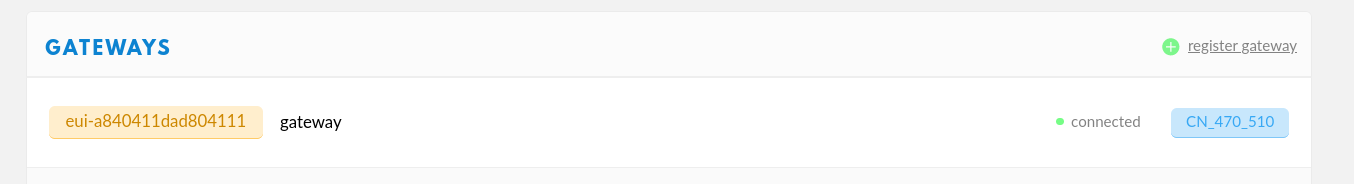
\includegraphics[width=\textwidth]{images/Quanh/Gateway_console.png}
        \caption{Giao diện Gateway đã được tạo (chưa connect)}
        \label{fig:gateway_console}
    \end{figure}
    \item Bước 3: Nhập ID vào Frequency plan tùy thuộc vào Gateway mà chọn cho phù hợp như hình \ref{fig:choose_gateway}, và kết quả được hiển thị ở hình \ref{fig:gateway_result} (nếu power on gateway thì status sẽ hiện "connected")
    \begin{figure}[H]
        \centering
        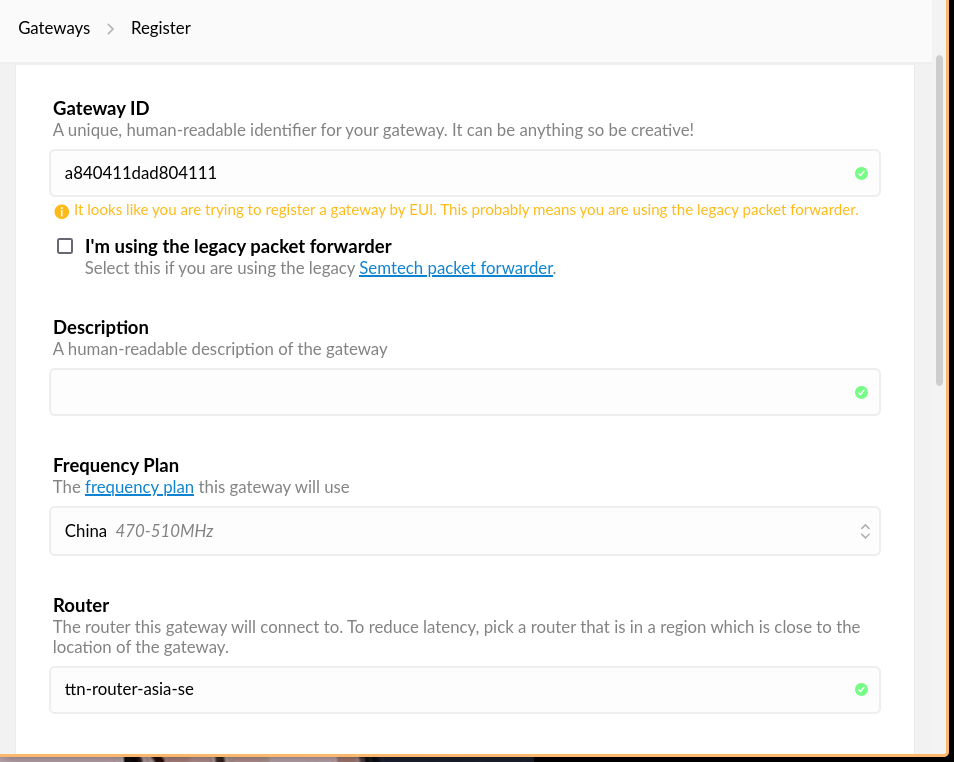
\includegraphics[width=\textwidth]{images/Quanh/Gateway_choose.png}
        \caption{Nhập ID vào Frequency plan}
        \label{fig:choose_gateway}
    \end{figure}
    \begin{figure}[H]
        \centering
        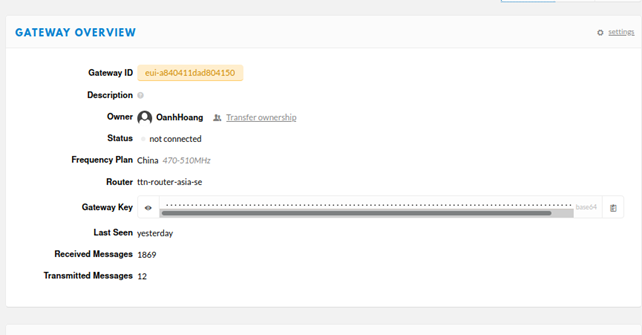
\includegraphics[width=\textwidth]{images/Quanh/Gateway_result.png}
        \caption{Overview khi đăng kí xong}
        \label{fig:gateway_result}
    \end{figure}
\end{description}
**do Gateway của nhóm sử dụng frequency 433Mhz nhưng The Things Network không hỗ trợ nên khi đăng kí sẽ là : china 470-510Mhz ( do tần số 433 trãi từng tần số 433 đến 510)

\subsection{Configure LG02 Gateway}
\begin{enumerate}
    \item Configure to LoRaWAN server:
    \begin{description}
        \item Bước 1: Config LG02 như hình \ref{fig:config_LG02}
        \begin{figure}[H]
            \centering
            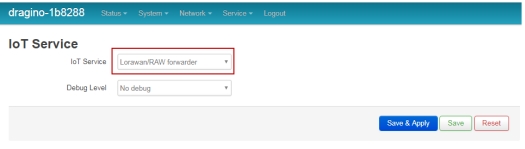
\includegraphics[width=\textwidth]{images/Quanh/Config_lg02.png}
            \caption{Config LG02}
            \label{fig:config_LG02}
        \end{figure}
        \item Bước 2: Chọn server address và gateway ID như hình \ref{fig:choose_server_address} (nhóm chọn ttn-router-asia-se)
        \begin{figure}[H]
            \centering
            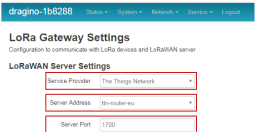
\includegraphics[width=\textwidth]{images/Quanh/Choose_server_address.png}
            \caption{Chọn server address thích hợp}
            \label{fig:choose_server_address}
        \end{figure}
    \end{description}

    \item Configure LG02's RX frequency: Ở frequency 433Mhz, có 8 channel uplink nhưng nhóm chọn channel 433.175Mhz để end-device join vào, thông sô như hình \ref{fig:radio_config}
    \begin{figure}[H]
        \centering
        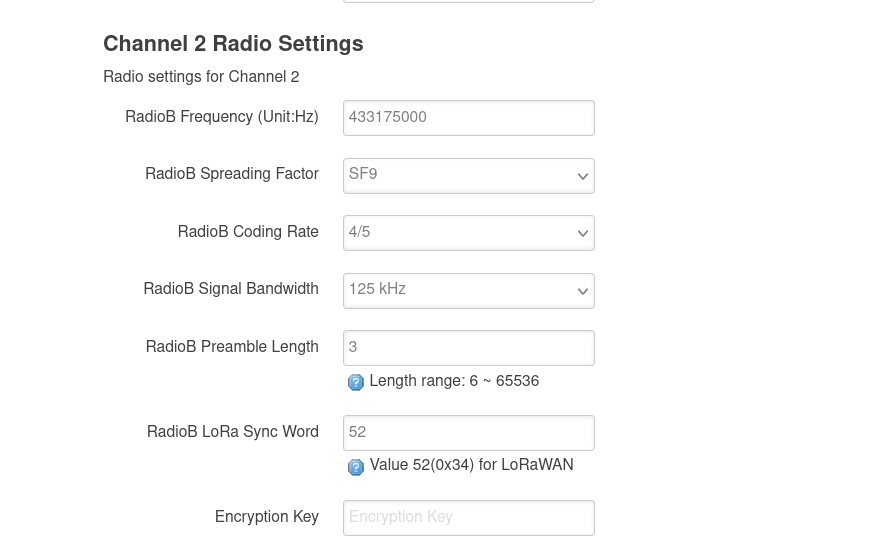
\includegraphics[width=\textwidth]{images/Quanh/Radio_config.png}
        \caption{Thông số configure}
        \label{fig:radio_config}
    \end{figure}
\end{enumerate}


\section{Setup End-Device}
\subsection{Thu gom rác}
Phần mềm sử dụng: Arduino IDE 1.8.2

Ngôn ngữ lập trình: C

Thiết bị Kit RF thu phát wifi Blue esp32 + Lora sx1278 oled Heltec.

\begin{description}
    \item Bước 1: Add lib esp32 từ link https://github.com/HelTecAutomation/Heltec\_ESP32 để thêm thư viện esp32 cho Arduino
    \item Bước 2: Add lib Lmic https://github.com/matthijskooijman/arduino-lmic để thêm vào thư viện Lmic cho Arduino
\end{description}

** Thư viện esp32 hỗ trợ hoạt động trên Heltech ESP32 develop framework.
** Thư viện Lmic cung cấp các giao tiếp LoRaWan ở classA và Class B. Tuy nhiên chỉ hỗ trợ ở band EU-868 và US 915. Nhưng thiết bị nhóm sử dụng là frequency 433Mhz nên cần sửa 1 số file để thiết bị có thể truyền data

Lúc này, có thể nạp code vào board như bình thường.

\subsection{Đăng kí trên TTN Server}
\begin{description}
    \item Bước 1: Tạo Application ID và handler như hình \ref{fig:create_application_id}, sau đó vào Devices → Register device → Điền Device ID
    \begin{figure}[H]
        \centering
        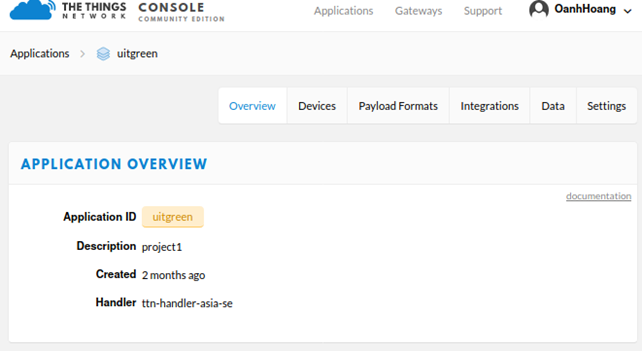
\includegraphics[width=\textwidth]{images/Quanh/Create_application_id.png}
        \caption{Tạo Application ID: uitgreen và handler: ttn-handler-asia-se}
        \label{fig:create_application_id}
    \end{figure}
    
    \item Bước 2: Sau khi đăng kí device thành công, The Things Network sẽ mặc định setup device join vào channel theo OTAA, nhưng nhóm chọn join theo ABP nên cần vào Setting → Activation method → ABP như hình \ref{fig:ABP_config}
    \begin{figure}[H]
        \centering
        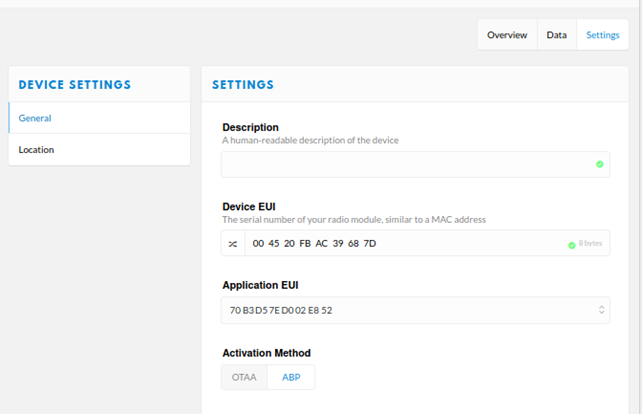
\includegraphics[width=\textwidth]{images/Quanh/ABP_config.png}
        \caption{Chọn phương thức ABP}
        \label{fig:ABP_config}
    \end{figure}
\end{description}

Sau khi đăng kí device thành công, thông tin device sẽ hiển thị như hình \ref{fig:device_profile} với Decoder như hình \ref{fig:device_decoder}
\begin{figure}[H]
    \centering
    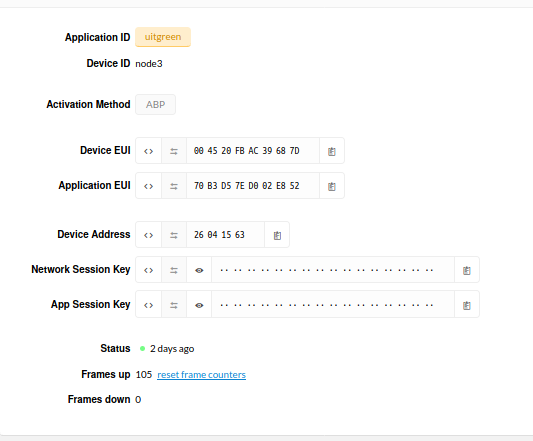
\includegraphics[width=\textwidth]{images/Quanh/Device_profile.png}
    \caption{Sau khi đăng kí device thành công}
    \label{fig:device_profile}
\end{figure}
\begin{figure}[H]
    \centering
    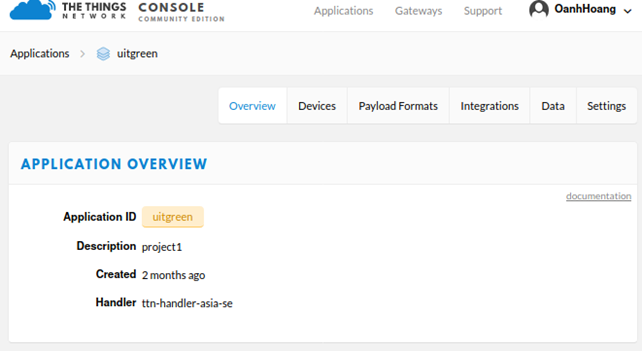
\includegraphics[width=\textwidth]{images/Quanh/Create_application_id.png}
    \caption{Decoder}
    \label{fig:device_decoder}
\end{figure}

** ở phần này Payload Formats sẽ tùy thuộc vào code nạp vào end-device

Nếu như end-device sử dụng thư viện Cayenne LPP để send data thì trên TTN phần Payload Formats sẽ như hình \ref{fig:payload_format}
\begin{figure}[H]
    \centering
    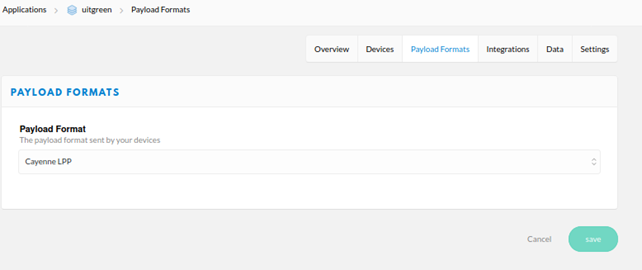
\includegraphics[width=\textwidth]{images/Quanh/Payload_format.png}
    \caption{Payload Formats: Cayenne LPP}
    \label{fig:payload_format}
\end{figure}

\subsection{So sánh khi sử dụng Cayenne LPP và Custom}

Ta có bảng \ref{tab.comparison.Cayenne}

\begin{table}[H]
    \centering
    \caption{Loại rác} 
    \label{tab.comparison.Cayenne}
    \begin{tabular}{| m{6cm} | m{6cm} |}
        \hline
        Cayenne LLP & Custom \\

        \hline
        •	Không cần decoder (do thư viện Cayenne LPP đã có những quy định về code ở end-device) & •	Cần decoder để TTN hiển thị thông tin \\
        •	Khó hiển thị thêm các trường data từ sensor khác (Vì chỉ  hỗ trợ mặc định cho sensor nhiệt độ độ ẩm, các sensor khác phải qua pin Analog) & •	Có thể thêm nhiều sensor dễ dàng bằng code trên node, và chỉ cần cài đặt Payload formats trên TTN để hiển thị thông tin \\
        •	Mặc định payload & •	Có thể thay đổi Payload \\
        
        \hline
    \end{tabular}
\end{table}

\subsection{Lưu ý khi nạp code cho node}

Vì sử dụng phương thức join vào server là ABP nên cần khai báo các thông tin cần thiết vào file *.ino để node có thể send data đến application server 

\begin{itemize}
    \item Device EUI, Network Session key và App Session key
    \item Để tối ưu việc truyền nhận từ node đến gateway,  nên disable các channels không cần thiết( chỉ enable channel đã khai báo ở RX của gateway)
\end{itemize}



